\documentclass {article}

% \usepackage{listings}

\usepackage{minted, xcolor, graphicx, caption, geometry}
% \usepackage{geometry}
% \definecolor{bg}{HTML}{282828}


\geometry{
  left=2.5cm,
  right=2.5cm,
  top=2.5cm,
  bottom=3cm
}
\captionsetup{font=footnotesize}


\begin {document}
\begin{figure}[t]
    \centering{
\includegraphics[scale=0.5]{logo.png}}
	\label{fig:logo}
\end{figure}
% \begintitlepage
% \centering
\author {Hugo Charels 000544051 \and Mickael Kovel 000396950}
\date {28 Avril 2023}
\title {Rapport de projet : Rectangle Tree}

% \subtitle "\
\includegraphics{logo.png}\\vspace{1cm}"
\maketitle
\newpage


\tableofcontents
\newpage
\section {Introduction}

% Les polygones jouent un rôle essentiel dans de nombreuses applications,
% qu'il s'agisse de représenter des régions administratives sur une carte, des informations géologiques,
% des zones dans des dessins vectoriels ou même des imageries médicales. Lors de la manipulation de telles données,
% une question courante se pose : à quel polygone appartient un point donné, tel qu'un clic de souris ou
% la position d'un capteur GPS ? Cette question est résolue par le problème du "Point in Polygon" (PIP),
% dont l'algorithme a été connu depuis 1962.
% \\
Dans de nombreuses applications, la manipulation de polygones est essentielle. Ces polygones peuvent représenter
des régions administratives, des informations géologiques, des zones de dessins vectoriels ou encore des
images médicales. Lorsqu'il s'agit de déterminer à quel polygone appartient un point donné, une question se pose :
comment résoudre efficacement le problème du "Point in Polygon" (PIP) ?

% \\
L'algorithme PIP, connu depuis 1962, consiste à compter le nombre de fois qu'une demi-droite partant du point
traverse une arête du polygone. Si ce nombre est pair, le point est à l'extérieur du polygone, sinon,
il est contenu à l'intérieur. Cependant, si l'on a des milliers de polygones complexes à tester avec un
grand nombre de points, une méthode naïve devient inefficace.

Une première optimisation consiste à utiliser l'enveloppe ou "minimum bounding rectangle" (MBR),
qui est le plus petit rectangle horizontal englobant totalement le polygone. Avant d'appliquer l'algorithme PIP,
on vérifie d'abord l'inclusion du point dans le MBR, ce qui permet de réduire le nombre d'appels à PIP.

Cependant, lorsque le nombre de polygones et de MBR est élevé, une approche hiérarchique basée sur l'algorithme R-Tree
devient pertinente. En regroupant les MBR de manière optimale, on peut éviter de considérer tous les MBR pour
chaque point à tester.

Dans ce projet, nous allons implémenter et évaluer deux variantes de l'algorithme R-Tree (quadratique et linéaire)
pour résoudre efficacement le problème du PIP. Nous testerons ces variantes avec différents paramètres pour
évaluer leurs performances.

Le rapport détaillera la méthodologie utilisée, les résultats obtenus et une analyse approfondie des performances
des variantes de l'algorithme R-Tree. Nous discuterons également des défis rencontrés et des perspectives pour de
futures recherches.


En conclusion, ce projet vise à résoudre efficacement le problème du PIP en utilisant l'algorithme
R-Tree.
Les résultats obtenus nous permettront de déterminer la meilleure variante en fonction des
paramètres et de formuler des recommandations pour d'éventuelles améliorations.

\section {Structure}

Dans cette section, nous allons explorer la structure d'un R-Tree, une arborescence utilisée
pour organiser efficacement les données géospatiales et résoudre le problème du
"Point in Polygon" (PIP). L'objectif est de comprendre comment cette structure hiérarchique
permet de regrouper les MBR (minimum bounding rectangles) de manière optimale.

Un R-Tree est une structure de données arborescente utilisée pour l'indexation spatiale des
objets géométriques. Il est conçu pour stocker et organiser efficacement des données
multidimensionnelles, telles que des polygones, des points ou des rectangles.

L'idée fondamentale d'un R-Tree est de regrouper les MBR de manière hiérarchique.
Chaque nœud de l'arbre représente un MBR, qui peut être un polygone ou un rectangle englobant
un groupe de MBR plus petits.
\begin{itemize}

    \item Nœuds internes : Les nœuds internes de l'arbre contiennent des MBR qui englobent
	plusieurs autres MBR.
	Ils servent de guides pour naviguer dans la structure et réduire la recherche de MBR
	pertinents lors de la résolution du problème du PIP.

    \item Feuilles : Les nœuds feuilles de l'arbre contiennent les MBR individuels et sont
	généralement associés à des objets géométriques spécifiques.
	Ils sont utilisés pour effectuer les tests d'inclusion du point lors de	la résolution
	du PIP.
\end{itemize}

L'algorithme R-Tree utilise des critères spécifiques pour regrouper les MBR de manière optimale.
Ces critères visent à maximiser la compacité des groupes de MBR et minimiser leur superposition
avec d'autres groupes.

\begin{itemize}
    \item Critère de regroupement spatial : Les MBR ayant une proximité spatiale élevée sont
	regroupés ensemble pour réduire la recherche dans les parties de l'arbre non pertinentes
	pour le point en cours d'évaluation.

    \item Critère de compacité : Lorsque plusieurs MBR sont candidats pour un regroupement,
	celui qui crée le MBR englobant le plus compact est préféré.
	Cela garantit une meilleure utilisation de l'espace de stockage et une réduction des
	opérations de recherche.

\end{itemize}
Nous détaillerons la recherche d'un point dans un R-Tree dans la section \ref{recherche}.

\section {Création}

Dans cette section, nous allons aborder la création d'un R-Tree, en expliquant les étapes de base
pour construire cette structure hiérarchique.
Nous présenterons également deux algorithmes de construction :
le split quadratique et le split linéaire.

La création d'un R-Tree implique de regrouper les MBR de manière hiérarchique.
Pour cela, nous commençons avec un ensemble de MBR individuels et suivons un processus
de division et de regroupement pour former l'arbre.

L'algorithme de construction de base utilise deux étapes principales : le split et le picknext.
Le split consiste à diviser un groupe de MBR en deux groupes plus petits,
tandis que le picknext sélectionne le prochain MBR à insérer dans l'arbre.

Il existe deux variantes d'algorithmes de split : le split quadratique et le split linéaire.
Explorons-les plus en détail.


\subsection {Split quadratique}
Le split quadratique est un algorithme de division utilisé dans la construction d'un R-Tree.
Il se base sur le concept de compacité des MBR pour choisir les MBR à diviser.

% L'idée du split quadratique est de sélectionner deux MBR initiaux qui englobent le plus grand espace possible.
% Pour cela, nous calculons toutes les paires possibles de MBR et choisissons celle qui crée les deux MBR les plus
% compacts.
L'idée du split quadratique est de sélectionner deux MBR initiaux qui sont le plus éloignés possible.
Pour cela, nous calculons toutes les paires possibles de MBR et choisissons celle qui dont
l'aire d'encadrement est la plus grande.

Avantages du split quadratique :

\begin{itemize}
    \item Il tend à créer une structure plus équilibrée en termes de taille des nœuds et de
	compacité des MBR.
    \item Il est moins susceptible de générer des feuilles surchargés ou des nœuds internes
	avec peu de MBR.

\end{itemize}
Inconvénients du split quadratique :

\begin{itemize}
    \item Il peut être plus coûteux en termes de temps de calcul, car il nécessite l'évaluation
	de toutes les paires de MBR possibles.
\end{itemize}

\subsubsection {Pick Seed}


Dans le contexte du split quadratique, le pickseed est l'algorithme utilisé pour choisir les
deux MBR initiaux à diviser.

L'algorithme du pickseed (quadratique) consiste à énumérer toutes les paires possibles de MBR et à sélectionner
celle qui a l'aire d'encadrement la plus grande.

L'objectif est de trouver les deux MBR qui englobent l'espace maximal, formant ainsi une base solide
pour la construction ultérieure de l'arbre.

% test
\begin{minted}{java}

protected AbstractNodePair pickSeeds(Node node) {
    AbstractNodePair nodes = new AbstractNodePair(node.getChild(0), node.getChild(1));
    double bestExpansion = 0;
    for (int i = 1; i < node.getChildren().size(); i++) {
        for (int j = i + 1; j < node.getChildren().size(); j++) {
            double expansion = node.getChild(i).getMBR().getExpansion(node.getChild(j).getMBR()) -
                node.getChild(j).getMBR().getArea();
            if (expansion > bestExpansion) {
                nodes.n1 = node.getChild(i);
                nodes.n2 = node.getChild(j);
                bestExpansion = expansion;
            }
        }
    }
    return nodes;
}

\end{minted}
% \end{lstlisting}


\subsubsection {Pick Next}

Après avoir choisi les deux MBR initiaux, le picknext est utilisé pour sélectionner le prochain MBR
à insérer dans l'arbre lors du processus de construction.

L'algorithme du picknext (quadratique) consiste à évaluer l'augmentation d'aire résultant de l'ajout de chaque MBR
restant. Le MBR qui entraîne la plus petite augmentation d'aire est choisi
comme prochain MBR à insérer.

Ce processus est répété jusqu'à ce que tous les MBR soient attribués à un groupe.
% \begin{lstlisting}[language=Java, caption=Algorithme du picknext]
% \begin{minted}[bgcolor=bg]{java}


\begin{minted}{java}

protected void pickNext(Node n1, Node n2, List<AbstractNode> children) {
    while(!children.isEmpty()) {
        AbstractNode best = null;
        Node father = null;
        double maxDelta = -1;
        for (AbstractNode node : children) {
            double n1Expansion = n1.getMBR().getExpansion(node.getMBR()) - node.getMBR().getArea();
            double n2Expansion = n2.getMBR().getExpansion(node.getMBR()) - node.getMBR().getArea();
            double delta = Math.abs(n1Expansion - n2Expansion);
            if (delta > maxDelta) {
                maxDelta = delta;
                best = node;
                if (n1Expansion < n2Expansion) { father = n1; }
                else { father = n2; }
            }
        }
        children.remove(best);
        father.addChild(best);
        father.expandMBR(best.getMBR());
    }
}
\end{minted}



\subsection {Split linéaire}

Le split linéaire est un autre algorithme de division utilisé dans la construction d'un R-Tree.
% Il ne prend pas en compte la compacité des MBR lors de la sélection des MBR à diviser.
% mais se base sur la position des MBR. Ce qui permet de réduire le temps de calcul.

% Le split linéaire est une autre variante de l'algorithme de division utilisé dans la construction d'
% un R-Tree.
Contrairement au split quadratique, il ne prend pas en compte la compacité des MBR lors de la
sélection des MBR à diviser mais se base sur la position relative des MBR les uns par rapport
aux autres.
Ce qui permet de réduire le temps de calcul.

L'idée du split linéaire est de sélectionner deux MBR initiaux qui sont le plus extrêmes possible.

Avantages du split linéaire :

\begin{itemize}
    \item Il est plus rapide que le split quadratique, car il ne nécessite pas l'évaluation de
	toutes les paires de MBR possibles.
    \item Il est plus simple à implémenter.

\end{itemize}
Inconvénients du split linéaire :

\begin{itemize}
    \item Il tend à créer une structure moins équilibrée en termes de taille des nœuds et de
	compacité des MBR.
    \item Il est plus susceptible de générer des feuilles surchargés ou des nœuds internes
	avec peu de MBR.

\end{itemize}

\subsubsection {Pick Seed}

Le pickseed (linéaire) est utilisé pour sélectionner les deux MBR initiaux dans le contexte du split linéaire.
Il s'agit simplement d'attribuer les deux premiers MBR qui ont leurs positions situées aux extrémités.
Pour cela, nous retenons deux paires de MBR, une dont les positions extrêmes concernent l'axe des abscisses et
l'autre l'axe des ordonnées.
La paire choisie est celle dont la noramlisation de la distance est la plus grande.



\begin{minted}{java}
protected AbstractNodePair pickSeeds(Node node) {
    List<AbstractNode> children = new java.util.ArrayList<>(node.getChildren());

    AbstractNode nodeMinOfMaxX = children.stream().min(
	    Comparator.comparingDouble(n -> n.getMBR().getXMax())).orElse(null);
    AbstractNode nodeMaxOfMinX = children.stream().max(
	    Comparator.comparingDouble(n -> n.getMBR().getXMin())).orElse(null);
    AbstractNode nodeMinOfMaxY = children.stream().min(
	    Comparator.comparingDouble(n -> n.getMBR().getYMax())).orElse(null);
    AbstractNode nodeMaxOfMinY = children.stream().max(
	    Comparator.comparingDouble(n -> n.getMBR().getYMin())).orElse(null);

    double smallDistX = nodeMaxOfMinX.getMBR().getXMax() - nodeMinOfMaxX.getMBR().getXMin();
    double bigDistX = nodeMaxOfMinX.getMBR().getXMin() - nodeMinOfMaxX.getMBR().getXMax();
    double smallDistY = nodeMaxOfMinY.getMBR().getYMax() - nodeMinOfMaxY.getMBR().getYMin();
    double bigDistY = nodeMaxOfMinY.getMBR().getYMin() - nodeMinOfMaxY.getMBR().getYMax();
    if (smallDistX/bigDistX > smallDistY/bigDistY)
	return new AbstractNodePair(nodeMinOfMaxX, nodeMaxOfMinX);
    else
	return new AbstractNodePair(nodeMinOfMaxY, nodeMaxOfMinY);

}
\end{minted}

\subsubsection {Pick Next}

Le picknext (linéaire) est utilisé pour sélectionner le prochain MBR à insérer dans l'arbre lors de la construction.
Il suffit de choisir le prochain MBR dans l'ordre de leur apparition lors du parcours.


\begin{minted}{java}
private void pickNext(Node n1, Node n2, List<AbstractNode> children) {
    for (AbstractNode child : children) {
	if (n1.getMBR().getExpansion(child.getMBR()) <
		n2.getMBR().getExpansion(child.getMBR())) {
	    n1.addChild(child);
	    n1.expandMBR(child.getMBR());
	}
	else {
	n2.addChild(child);
	n2.expandMBR(child.getMBR());
	}
    }
}
\end{minted}

\subsection {Split suspicieux}
Nous avons implémenté un algorithme de split suspicieux qui est une variante du split linéaire.
Il se différencie du split linéaire de l'algorithme de Guttman par le choix des MBR à diviser.

\subsubsection {Pick Seed}
Le pickseed (suspicious) est utilisé pour sélectionner les deux MBR initiaux dans le contexte du split suspicieux.
Il s'agit simplement d'attribuer les deux premiers MBR qui ont leurs positions situées aux extrémités.
Pour cela, nous retenons les quatres MBR dont les positions extrêmes concernent l'axe des abscisses et 
l'axe des ordonnées.
Nous appelons à ce moment la fonction pickseed (quadratique).
Dans ce cadre, la fonction pickseed (quadratique) est linéaire car elle ne prend en compte que les quatres MBR
\subsubsection {Pick Next}



\section {Recherche}\label{recherche}



La recherche dans un R-Tree est l'une des fonctionnalités clés de cette structure de données.
Elle permet de déterminer à quel nœud ou à quel objet géométrique correspond un point donné.
L'algorithme de recherche dans un R-Tree repose sur le principe de parcours de l'arbre.

L'algorithme find, présenté ci-dessous, effectue une recherche d'un point p dans un R-Tree :


\begin{minted}{java}
public LeafData find(Point p) {
    Queue<AbstractNode> queue = new LinkedList<AbstractNode>();
    queue.add(root);
    BiConsumer<Node, Queue<AbstractNode>> addChildrenToQueue = (n, q) ->
        n.getChildren().stream().filter(child -> child.getMBR().contains(p)).forEach(q::add);
    while (!queue.isEmpty()) {
	AbstractNode temp = queue.poll();
	if (temp.isLeaf()) {
	    if (((Leaf)temp).getDataPolygon().contains(p)){
		return (Leaf) temp;
	    } else { continue; }
	}
	addChildrenToQueue.accept((Node) temp, queue);
    }
    return null;
}
\end{minted}

L'algorithme find utilise une file d'attente (queue) pour effectuer un parcours en largeur de l'arbre.
Il commence par ajouter le nœud racine à la file d'attente. Ensuite, il itère tant que la file d'attente
n'est pas vide. À chaque itération, il récupère un nœud de la file d'attente et effectue les actions suivantes :

\begin{itemize}
    \item Si le nœud est une feuille (Leaf), il vérifie si le polygone de données de la feuille contient le point
	recherché. Si c'est le cas, il renvoie la feuille.
	Sinon, il continue le parcours.
    \item Si le nœud est un nœud interne (Node), il ajoute ses enfants dont les MBR contiennent le point
	recherché à la file d'attente en utilisant la fonction addChildrenToQueue.
	Cette fonction filtre les enfants du nœud en ne gardant que ceux dont le MBR (Minimum Bounding Rectangle)
	contient le point recherché, puis les ajoute à la file d'attente.
    \item Si aucune feuille ne correspond au point recherché, la fonction renvoie null.
\end{itemize}

L'algorithme find garantit que tous les nœuds qui contiennent potentiellement le point sont visités de manière
efficace, en évitant de parcourir les nœuds qui ne sont pas pertinents.

Cette fonction de recherche sera mise en œuvre dans le cadre du projet pour effectuer des recherches
de points dans les R-Trees construits et évaluer leur performance.



\section {Expériences sur donnees réelles}


Pour évaluer les performances de l'algorithme de recherche dans un R-Tree,
nous avons réalisé des expérimentations en utilisant des données réelles.
Nous avons utilisé les ensembles de données suivants :

\begin{itemize}

    \item Belgique - Secteur. Voir \ref{belgique}
    \item France - Communes. Voir \ref{france}
    \item Monde - Pays. Voir \ref{mondePays}
    \item Monde - Villes. Voir \ref{mondeVilles}
\end{itemize}

Nous avons construit des arbres R-Tree à la fois en utilisant l'algorithme de partitionnement quadratique
et l'algorithme de partitionnement linéaire.

Ensuite, nous avons effectué des recherches en utilisant un ensemble de 5000 points de recherche différents
dans chaque jeu de données afin d'obtenir les résultats correspondants.
% Nous effectuons une moyenne des temps de recherche qui est calculée en faisant ces 1000 recherches 5 fois 
% pour chaque jeu de données et chaque algorithme de split.

Nous recommençons l'expérience en faisant varier le nombre maximum d'enfants par nœud allant de 2 au nombre
maximum de polygones par jeu de données par pas de nbPolygones/20.

Nous porterons ces données sur un graphique afin de pouvoir comparer les performances des deux types d'arbres,
avec en abscisse le nombre maximum de polygones par nœud et en ordonnée le temps de recherche pour 5000 points
en millisecondes.
De plus, nous avons porté de la même manière les temps de construction des arbres en fonction du nombre maximum
de polygones par nœud.

% Enfin, nous avons calculé le temps moyen de recherche pour chaque jeu de données et chaque algorithme de split.
% (voir \ref{analyse})

Les résultats de ces expérimentations nous permettent de comparer les performances des deux types d'arbres
(quadratique et linéaire) en termes de temps de construction et d'exécution des recherches.

\subsection {Belgique - Secteurs statistiques}\label{belgique}

\begin{figure}[h]
    \begin{minipage}[t]{0.46\textwidth}
	\centering
	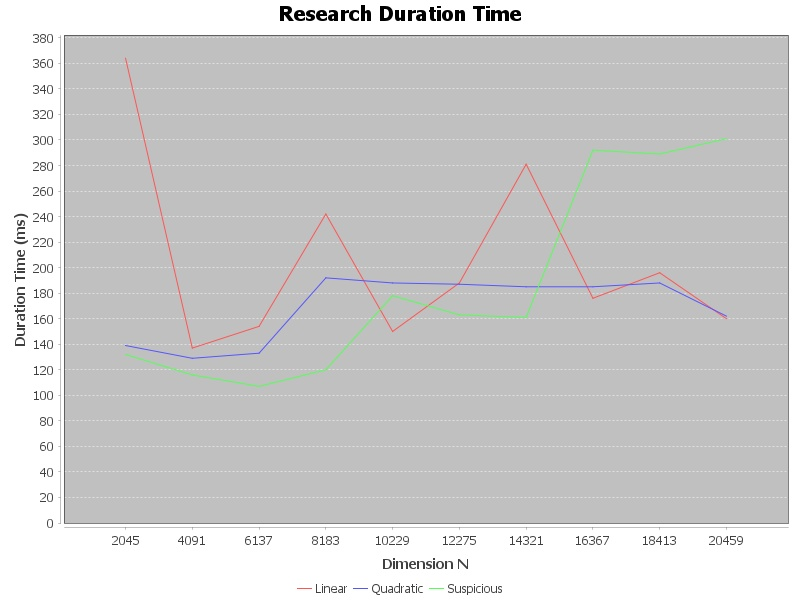
\includegraphics[width=\textwidth]{research_graph_belgium.png}
	\caption{Temps de recherche en fonction du nombre de polygones par noeud}
	\label{fig:belgique_stat_find_lin}
    \end{minipage}
    \begin{minipage}[t]{0.46\textwidth}
	\centering
	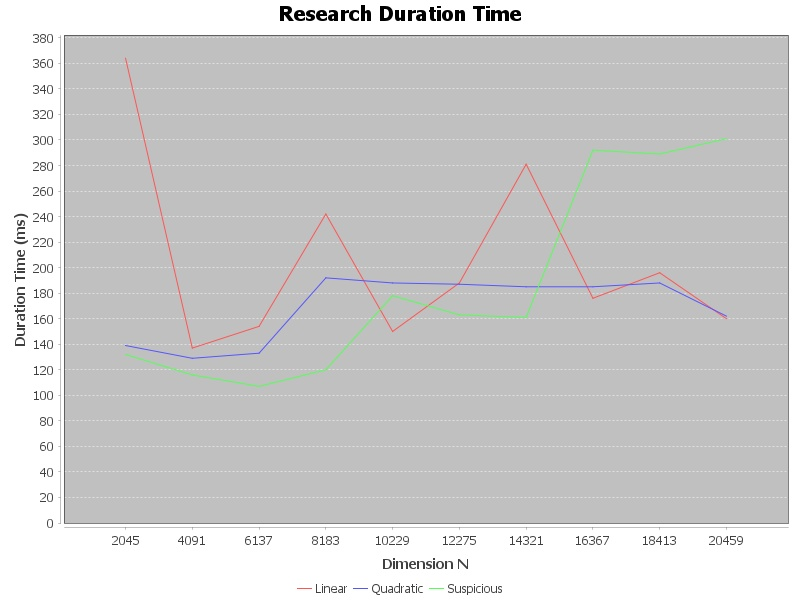
\includegraphics[width=\textwidth]{research_graph_belgium.png}
	\caption{Temps de recherche en fonction du nombre de polygones par noeud}
	\label{fig:belgique_stat_find_quad}
    \end{minipage}
\end{figure}

    % \centering{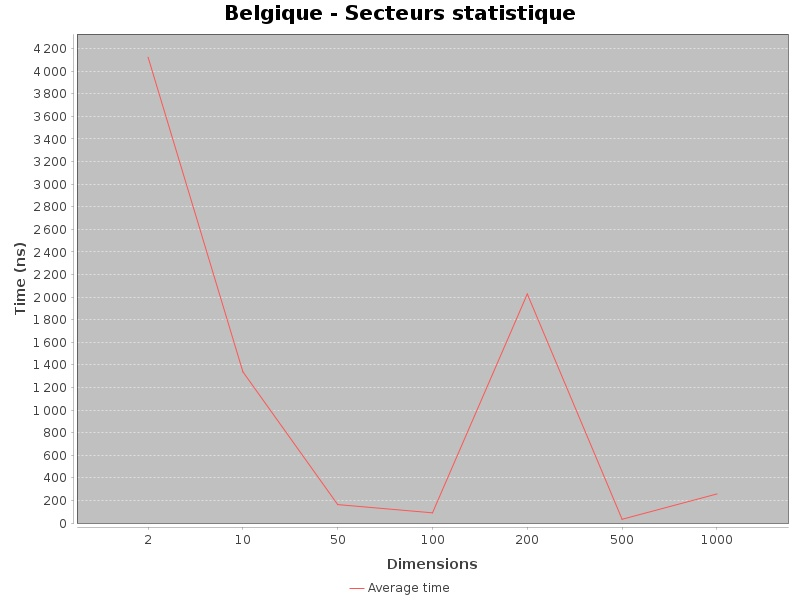
\includegraphics[scale=0.3]{graph_lineaire_Belgique.png}}
	% \label{fig:belgique_stat_find_lin}
% \end{figure}
% \begin{figure}[t]
%     \centering{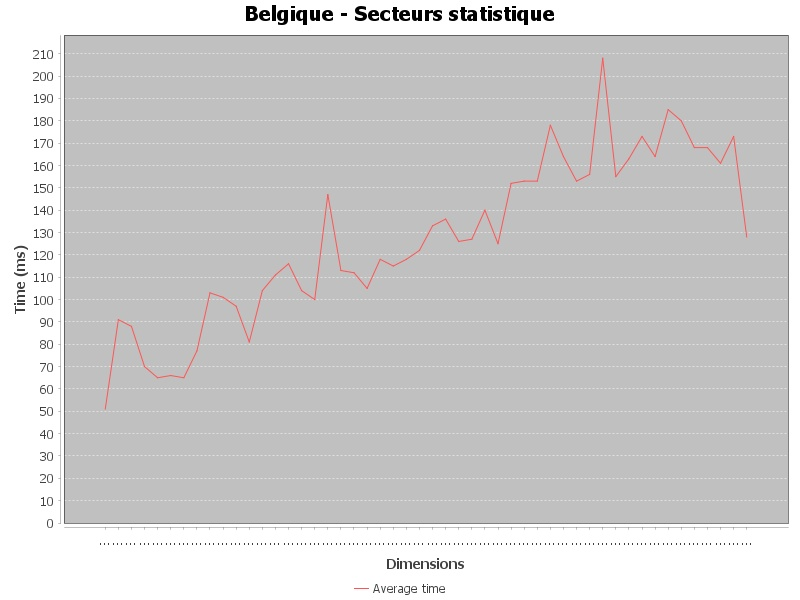
\includegraphics[scale=0.5]{graph_quadratique_Belgique.png}}
% 	\label{fig:belgique_stat_find_quad}
% \end{figure}

\newpage
\subsection {France - Communes}\label{france}

\begin{figure}[h]
    \begin{minipage}[t]{0.46\textwidth}
	\centering
	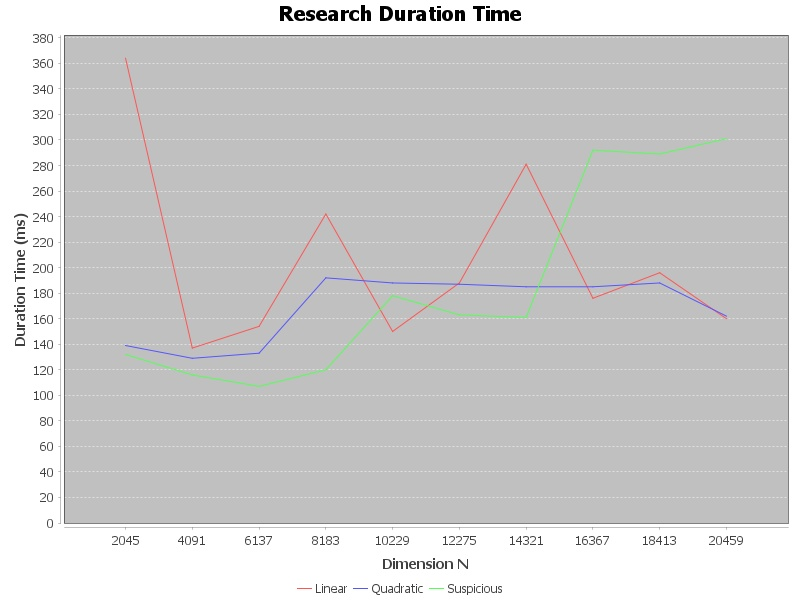
\includegraphics[width=\textwidth]{research_graph_belgium.png}
	\caption{Temps de recherche en fonction du nombre de polygones par noeud}
	\label{fig:belgique_stat_find_lin}
    \end{minipage}
    \begin{minipage}[t]{0.46\textwidth}
	\centering
	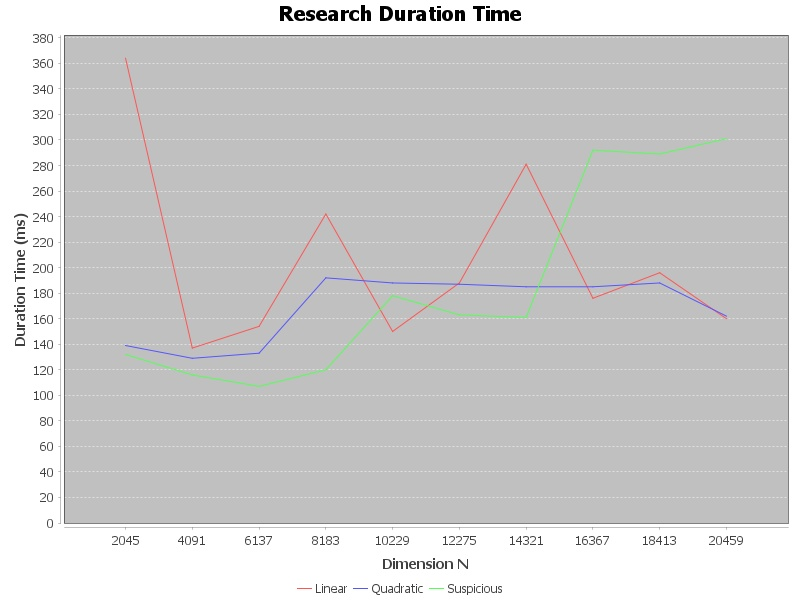
\includegraphics[width=\textwidth]{research_graph_belgium.png}
	\caption{Temps de recherche en fonction du nombre de polygones par noeud}
	\label{fig:belgique_stat_find_quad}
    \end{minipage}
\end{figure}
% \begin{figure}[t]
%     \centering{
\includegraphics[scale=0.5]{logo.png}}
% 	\label{fig:logo}
% \end{figure}

\subsection {Monde - Pays}\label{mondePays}

\begin{figure}[h]
    \begin{minipage}[t]{0.46\textwidth}
	\centering
	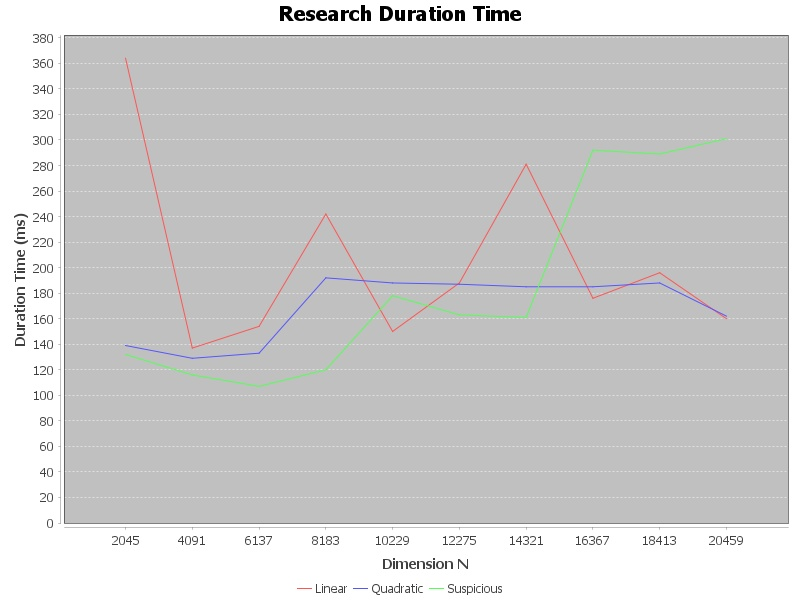
\includegraphics[width=\textwidth]{research_graph_belgium.png}
	\caption{Temps de recherche en fonction du nombre de polygones par noeud}
	\label{fig:belgique_stat_find_lin}
    \end{minipage}
    \begin{minipage}[t]{0.46\textwidth}
	\centering
	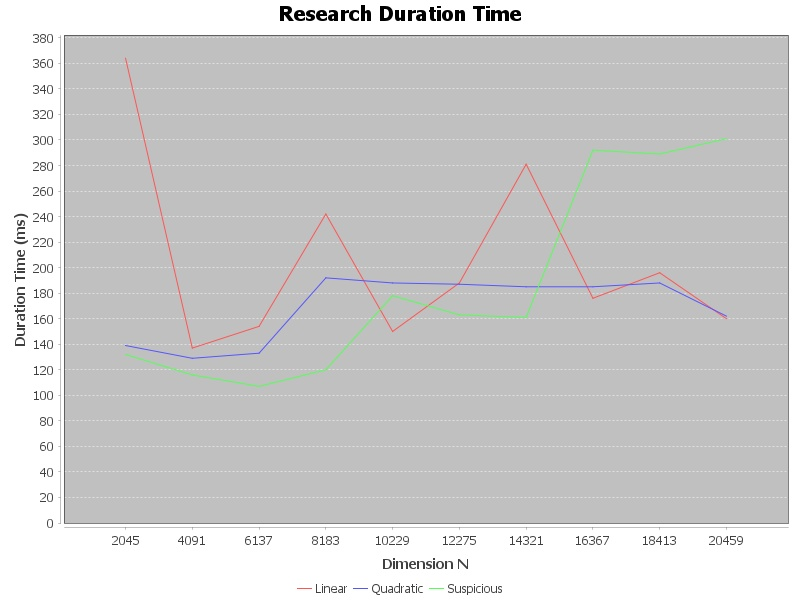
\includegraphics[width=\textwidth]{research_graph_belgium.png}
	\caption{Temps de recherche en fonction du nombre de polygones par noeud}
	\label{fig:belgique_stat_find_quad}
    \end{minipage}
\end{figure}

% \begin{figure}[t]
%     \centering{
\includegraphics[scale=0.5]{logo.png}}
% 	\label{fig:logo}
% \end{figure}
\newpage
\subsection {Monde - Villes}\label{mondeVilles}
\begin{figure}[h]
    \begin{minipage}[t]{0.46\textwidth}
	\centering
	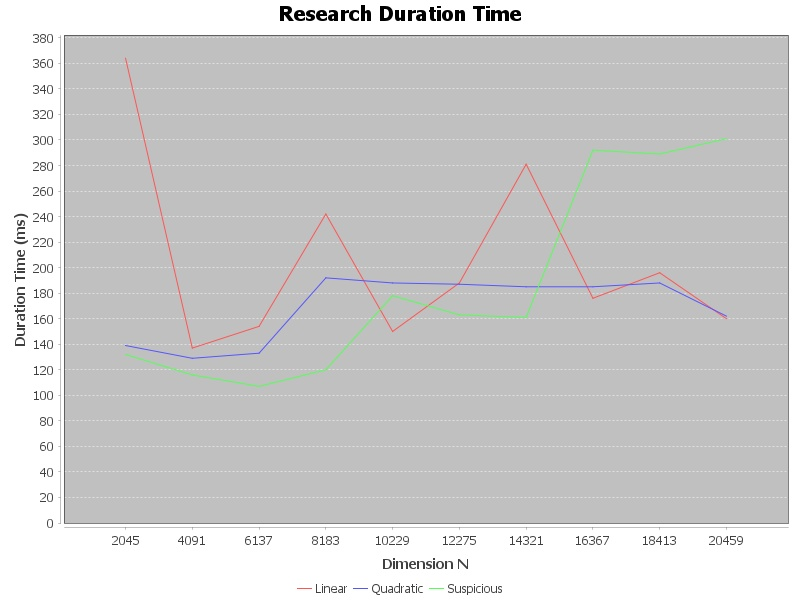
\includegraphics[width=\textwidth]{research_graph_belgium.png}
	\caption{Temps de recherche en fonction du nombre de polygones par noeud}
	\label{fig:belgique_stat_find_lin}
    \end{minipage}
    \begin{minipage}[t]{0.46\textwidth}
	\centering
	% 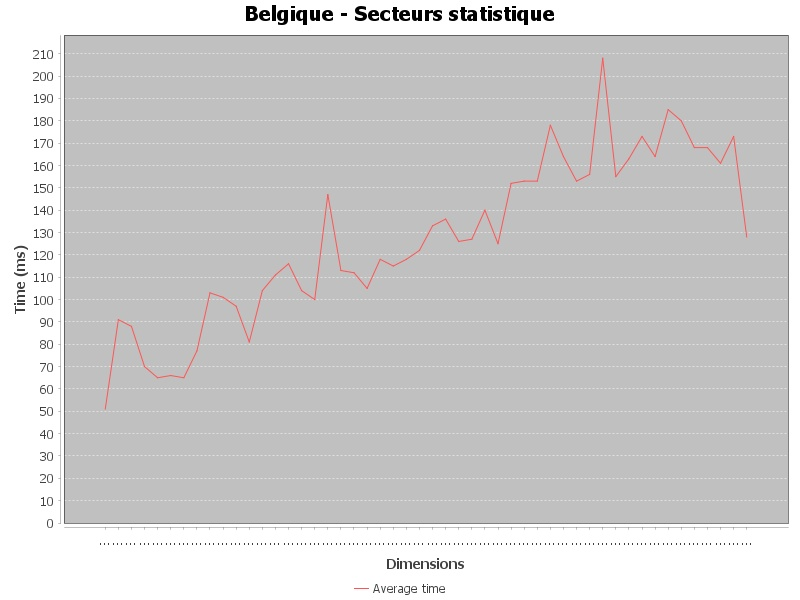
\includegraphics[width=\textwidth]{graph_quadratique_Belgique.png}
	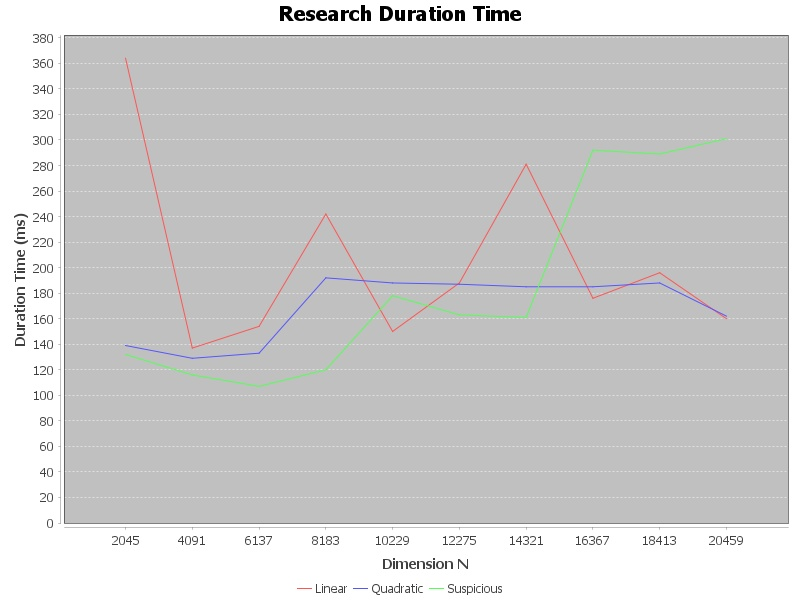
\includegraphics[width=\textwidth]{research_graph_belgium.png}
	\caption{Temps de recherche en fonction du nombre de polygones par noeud}
	\label{fig:belgique_stat_find_quad}
    \end{minipage}
\end{figure}

% \begin{figure}[t]
%     \centering{
\includegraphics[scale=0.5]{logo.png}}
% 	\label{fig:logo}
% \end{figure}
\subsection {Analyse}\label{analyse}
ici on va ecrire l'analyse

\section {Conclusion}
ici on va ecrire la conclusion

\section {Références bibliographiques}
ici on va ecrire les references bibliographiques




\end {document}
